\newpage
\section{Sprint 4 - Summary}

Due to limited resources and no working fixed pitch quadcopter, the team utilized the resources available. The group borrowed a set of DJI E600 motors with 12 inch propellers and assembled them on a new laser-cut plywood quadcopter (Fig. \ref{fig:plywood} \& \ref{fig:actual}). Our intentions was never to make such a big quadcopter, and had initially limited the propeller size to no more than 11 inches. Less than 11 inches was chosen in order to make a quadcopter that is easier to fly indoors and suitable in KIC facilities. At this stage, with limited time and resources to buy new hardware for fixed pitch, we chose to build it in order to have a working quadcopter to test code and actual flight.

\begin{figure}[h]
        \centering
         \begin{minipage}[b]{0.4\textwidth}
            \includegraphics[width = 1\textwidth]{VAPIQ-PICTURES/FixedPitchRender}
              \caption{SolidWorks model}
            \label{fig:plywood}
        \end{minipage}
        \hfill
        \begin{minipage}[b]{0.4\textwidth}
            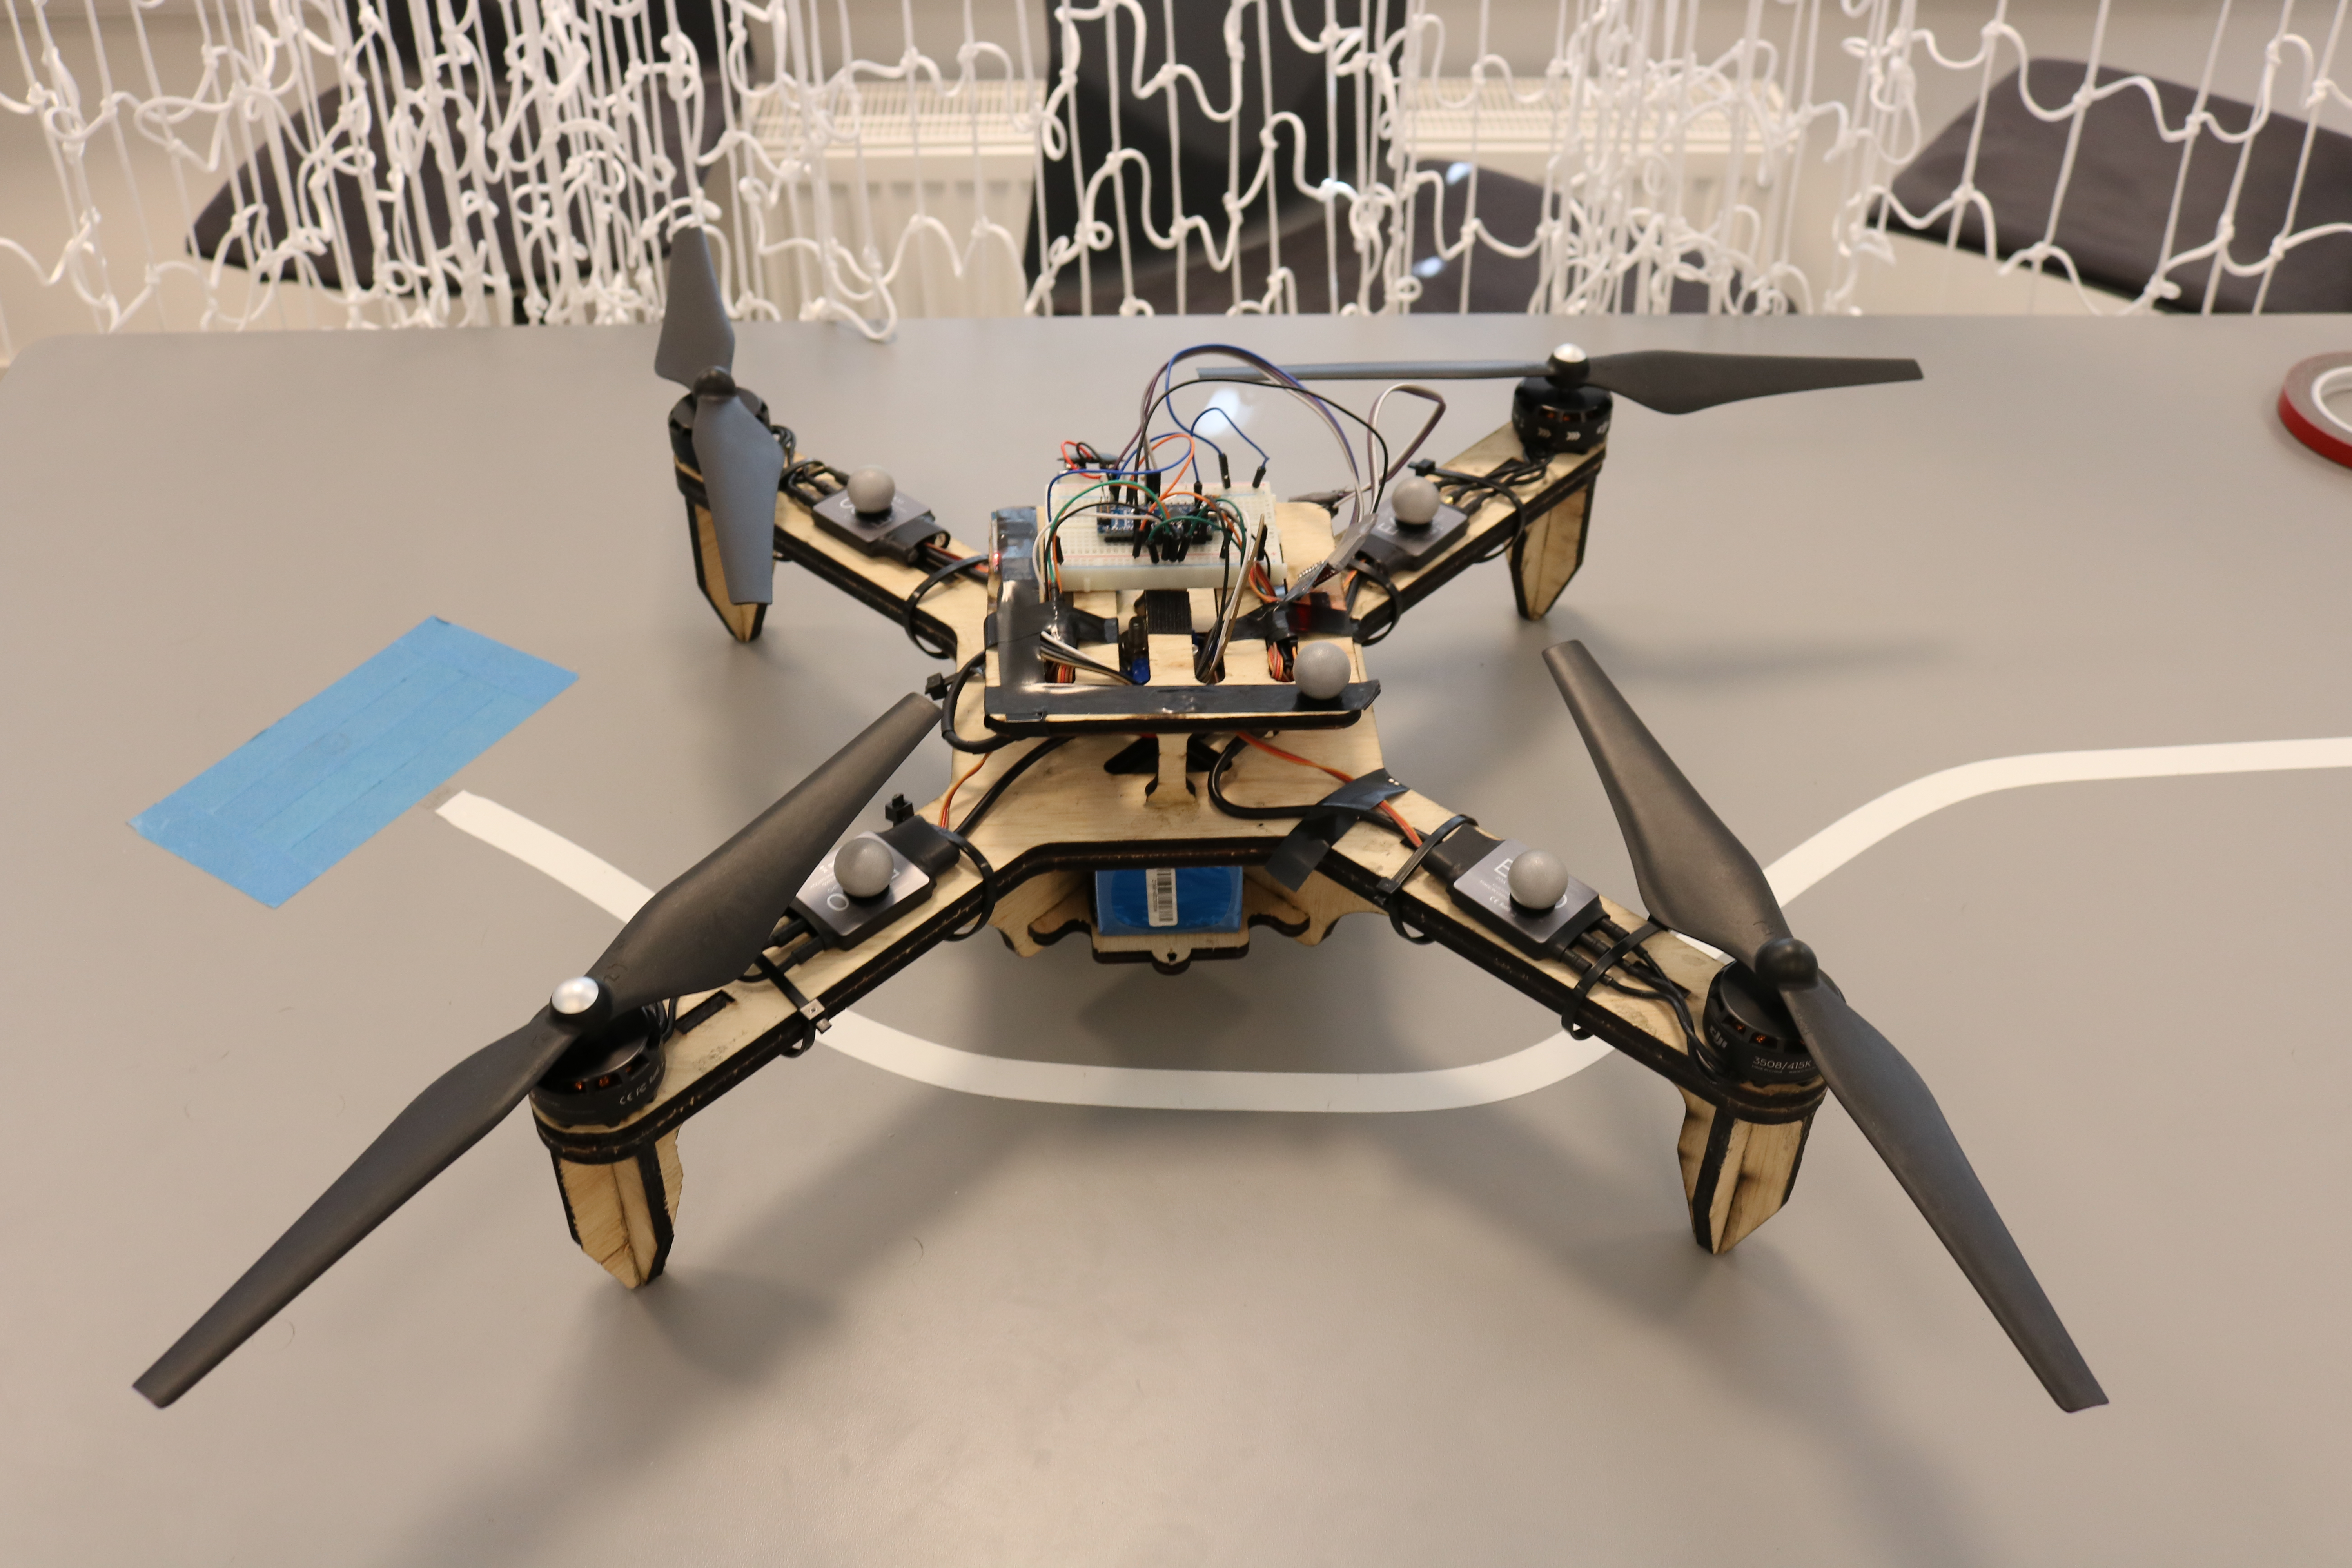
\includegraphics[width = \textwidth]{VAPIQ-PICTURES/FirstFixedPitch}
            \caption{Actual Model}
            \label{fig:actual}
        \end{minipage}
\end{figure}

In sprint 4, the group established stable communication with Qualisys and the PC, and can now send multiple data as one packet and decompose it on the Arduino. This will enable us to do the computing off-board with less delay, currently we are able to send data at least 10 times per second. The arming sequence for the ESCs is also improved and we do not need to spin the motors through all the activation values to arm. \\
\\
After assembly, the fixed pitch quadcopter has had its first flight. The flight-controller was very unstable, but after some testing we realized that there were a few minor logical faults in the code, both in the PID and in the IMU. We were recommended to use an IMU called MPU-9250 from a master student with experience in flight controllers. This IMU was difficult to use, but after a couple of days the team managed to reduce the noise, and the data seemed to be more correct than the 6050 IMU used earlier.
\\
\subsection{Completion and Scope Change}

In sprint 4, 98\% of all planned tasks were completed and we had a scope change of -6\% in total (Fig. \ref{fig:bds4}). The negative scope change is due to some tasks which were duplicated in sprint planning.

Project plan status, sprint 4:
        
    \begin{itemize}
        \item Prototype, Variabel Pitch, \textbf{Done} (Mechanisms produced to little thrust and quadcopter was to heavy)
        \item Matlab and Simulink Simulation, \textbf{Postponed}
        \item Stabilization And Regulation, \textbf{In progress}
        \item Tweak Flight Controller, Fixed Pitch, \textbf{In progress}
    \end{itemize}
        
        

\begin{figure}[h]
    \centering
         \includegraphics[width = 1\textwidth]{VAPIQ-PICTURES/BDSprint4}
      \caption{Sprint 4 - Burndown Chart}
    \label{fig:bds4}
\end{figure} 


\subsection{Results and Conclusions}

One of the biggest challenges in sprint 4 was noise and disturbance in the IMU. This caused us to use a lot of time on calibration and getting stable sensor data.

